\documentclass{article}
\usepackage[left=2cm,right=2cm,top=2cm,bottom=2cm]{geometry} 
\usepackage{blindtext}
\usepackage{graphicx} 
\usepackage[section]{placeins} 
\usepackage[spanish]{babel}
\usepackage{listings} 
\usepackage{xcolor} 
\usepackage{pdfpages}
\setcounter{secnumdepth}{2}

\newcommand*\rbreak{\par\noindent\linebreak}
\graphicspath{{/home/renato/screenshots/math/t3/}}

\begin{document}
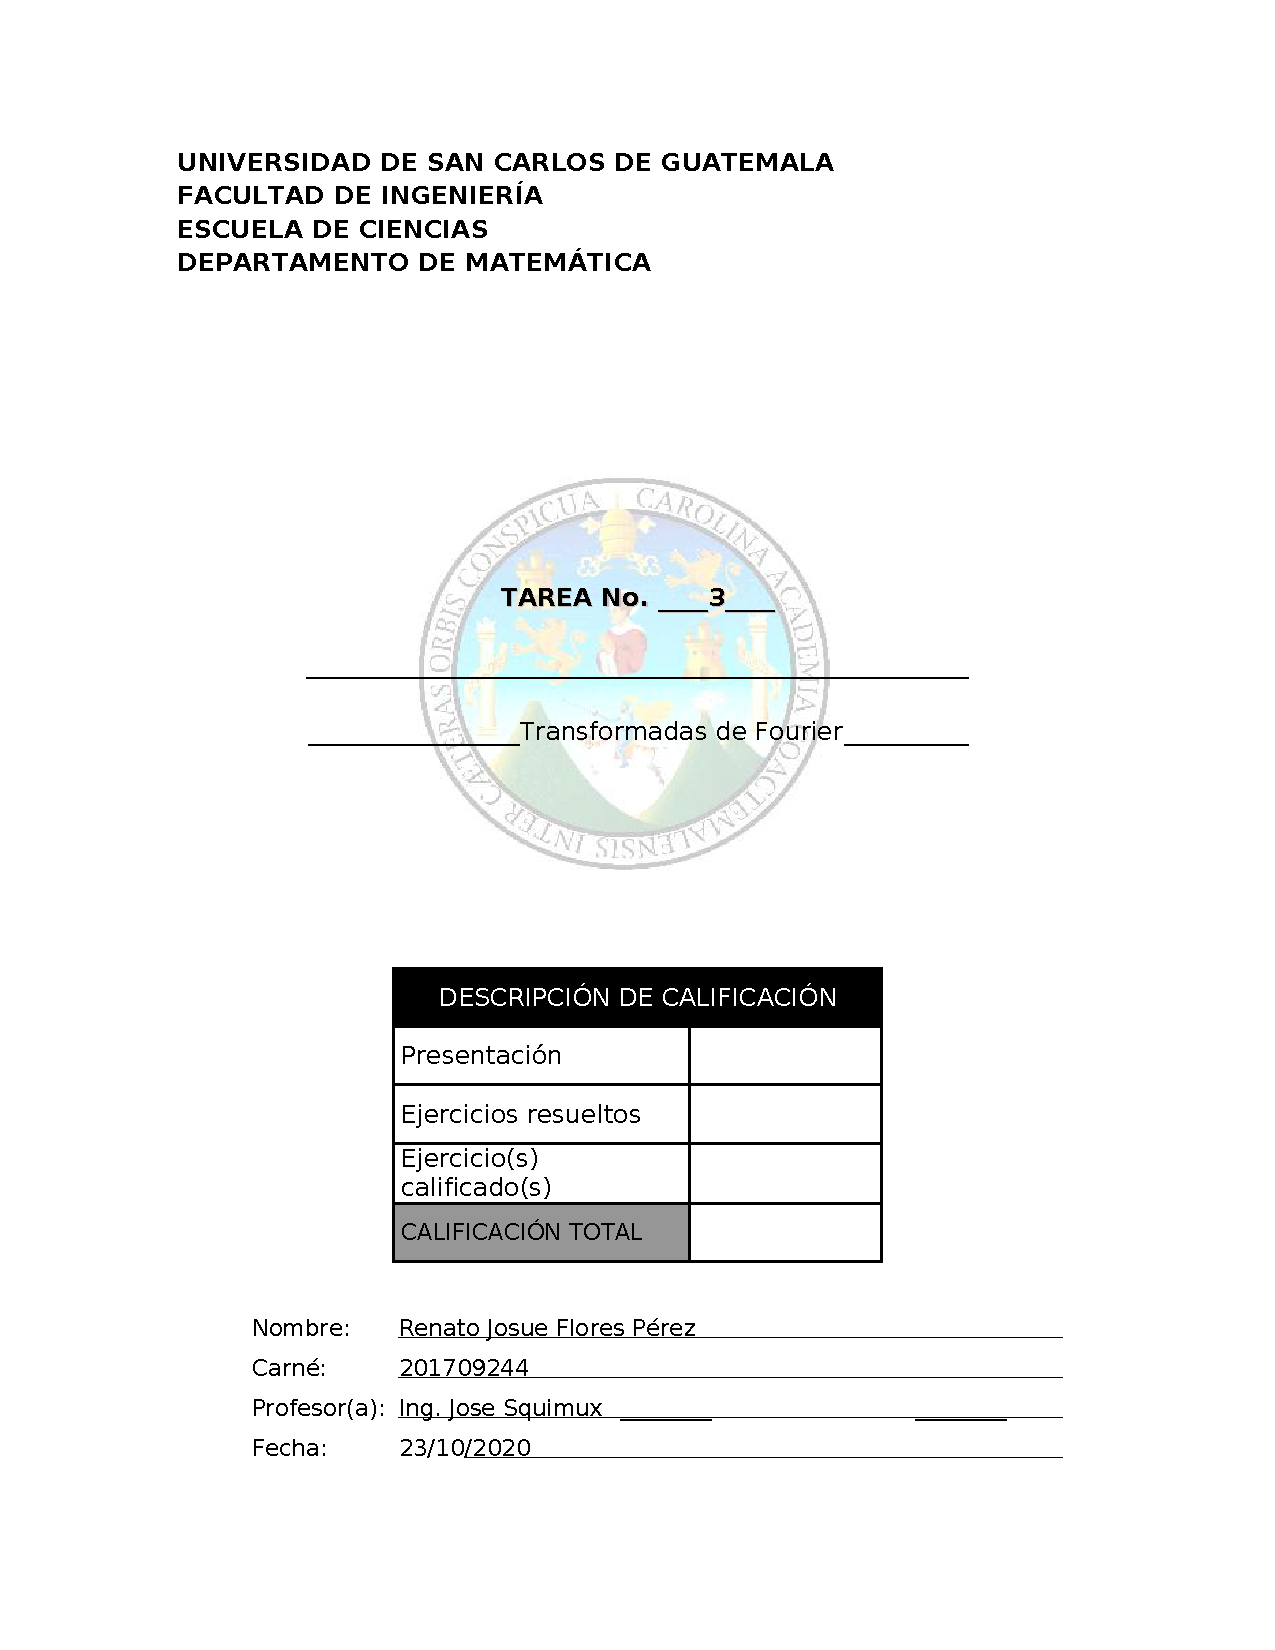
\includepdf{/home/renato/math/caratula.pdf}	
\includepdf[pages={1-}]{/home/renato/screenshots/math/t3/procedure.pdf}		
\pagebreak	
\section{Apendices}
	\begin{figure}[h]
	\includegraphics[width=\textwidth,keepaspectratio]{ej_7_1.png}
		 \caption{Ejercicio correlativo 7, inciso 1. \rbreak
		 Espectro de amplitud para 
		 $ F(w) = \frac{2 \, \sin\left(\omega\right)}{\omega} $ }
	\end{figure}
	\clearpage
	
	\begin{figure}[h]
	\includegraphics[width=\textwidth,keepaspectratio]{ej_7_2.png}
		 \caption{Ejercicio correlativo 7, inciso 2. \rbreak
		 Espectro de fase para 
		 $ F(w) = \frac{2 \, \sin\left(\omega\right)}{\omega} $ }
	\end{figure}
	\clearpage

	\begin{figure}[h]
	\includegraphics[width=\textwidth,keepaspectratio]{ej_8.png}
		 \caption{Ejercicio correlativo 8. \rbreak
		 Espectro de Amplitud para
		 $ F\{ f(t) cos(t) \}  $}
	\end{figure}
	\clearpage

	\begin{figure}[h]
	\includegraphics[width=\textwidth,keepaspectratio]{ej_9_1.png}
		 \caption{Ejercicio correlativo 9, inciso 1. \rbreak
		 Espectro de amplitud para 
		 $ F(w) = -\frac{2 \, {\left(\cos\left(\omega\right) - 1\right)}}{\omega^{2}} $ }
	\end{figure}
	\clearpage
	
	\begin{figure}[h]
	\includegraphics[width=\textwidth,keepaspectratio]{ej_9_3.png}
		 \caption{Ejercicio correlativo 9, inciso 3. \rbreak
		 Espectro de Amplitud comparando F(w) original y F(w) 
		 luego de aplicar el filtro }
	\end{figure}
	\clearpage
	
	\begin{figure}[h]
	\includegraphics[width=\textwidth,keepaspectratio]{ej_18_1.png}
		 \caption{Ejercicio correlativo 18. \rbreak
		 Grafica del espectro de Amplitud de Q(w)}
	\end{figure}
\clearpage
\section{Cursos aprobados del Área de Matemática}

\end{document}
